\documentclass[a4paper, 12pt]{article}
\usepackage[utf8]{inputenc}
\usepackage[english, ukrainian]{babel}

\usepackage{amsmath, amssymb}
\usepackage{multicol}
\usepackage{graphicx}
\usepackage{float}

\allowdisplaybreaks
\setlength\parindent{0pt}
\numberwithin{equation}{subsection}

\usepackage{hyperref}
\hypersetup{unicode=true,colorlinks=true,linktoc=all,linkcolor=red}

\numberwithin{equation}{subsection}

\renewcommand{\bf}[1]{\textbf{#1}}
\renewcommand{\it}[1]{\textit{#1}}
\newcommand{\bb}[1]{\mathbb{#1}}
\renewcommand{\cal}[1]{\mathcal{#1}}

\renewcommand{\epsilon}{\varepsilon}
\renewcommand{\phi}{\varphi}

\DeclareMathOperator{\diam}{diam}
\DeclareMathOperator{\rang}{rang}
\DeclareMathOperator{\const}{const}

\newenvironment{system}{%
  \begin{equation}%
    \left\{%
      \begin{aligned}%
}{%
      \end{aligned}%
    \right.%
  \end{equation}%
}
\newenvironment{system*}{%
  \begin{equation*}%
    \left\{%
      \begin{aligned}%
}{%
      \end{aligned}%
    \right.%
  \end{equation*}%
}

\makeatletter
\newcommand*{\relrelbarsep}{.386ex}
\newcommand*{\relrelbar}{%
  \mathrel{%
    \mathpalette\@relrelbar\relrelbarsep%
  }%
}
\newcommand*{\@relrelbar}[2]{%
  \raise#2\hbox to 0pt{$\m@th#1\relbar$\hss}%
  \lower#2\hbox{$\m@th#1\relbar$}%
}
\providecommand*{\rightrightarrowsfill@}{%
  \arrowfill@\relrelbar\relrelbar\rightrightarrows%
}
\providecommand*{\leftleftarrowsfill@}{%
  \arrowfill@\leftleftarrows\relrelbar\relrelbar%
}
\providecommand*{\xrightrightarrows}[2][]{%
  \ext@arrow 0359\rightrightarrowsfill@{#1}{#2}%
}
\providecommand*{\xleftleftarrows}[2][]{%
  \ext@arrow 3095\leftleftarrowsfill@{#1}{#2}%
}
\makeatother

\newcommand{\NN}{\mathbb{N}}
\newcommand{\ZZ}{\mathbb{Z}}
\newcommand{\QQ}{\mathbb{Q}}
\newcommand{\RR}{\mathbb{R}}
\newcommand{\CC}{\mathbb{C}}

\newcommand{\Max}{\displaystyle\max\limits}
\newcommand{\Sup}{\displaystyle\sup\limits}
\newcommand{\Sum}{\displaystyle\sum\limits}
\newcommand{\Int}{\displaystyle\int\limits}
\newcommand{\Iint}{\displaystyle\iint\limits}
\newcommand{\Lim}{\displaystyle\lim\limits}

\newcommand*\diff{\mathop{}\!\mathrm{d}}

\newcommand*\rfrac[2]{{}^{#1}\!/_{\!#2}}


\title{{\Huge МАТЕМАТИЧНА ФІЗИКА}}
\author{Скибицький Нікіта}
\date{\today}

\usepackage{amsthm}
\usepackage[dvipsnames]{xcolor}
\usepackage{thmtools}
\usepackage[framemethod=TikZ]{mdframed}

\theoremstyle{definition}
\mdfdefinestyle{mdbluebox}{%
	roundcorner = 10pt,
	linewidth=1pt,
	skipabove=12pt,
	innerbottommargin=9pt,
	skipbelow=2pt,
	nobreak=true,
	linecolor=blue,
	backgroundcolor=TealBlue!5,
}
\declaretheoremstyle[
	headfont=\sffamily\bfseries\color{MidnightBlue},
	mdframed={style=mdbluebox},
	headpunct={\\[3pt]},
	postheadspace={0pt}
]{thmbluebox}

\mdfdefinestyle{mdredbox}{%
	linewidth=0.5pt,
	skipabove=12pt,
	frametitleaboveskip=5pt,
	frametitlebelowskip=0pt,
	skipbelow=2pt,
	frametitlefont=\bfseries,
	innertopmargin=4pt,
	innerbottommargin=8pt,
	nobreak=true,
	linecolor=RawSienna,
	backgroundcolor=Salmon!5,
}
\declaretheoremstyle[
	headfont=\bfseries\color{RawSienna},
	mdframed={style=mdredbox},
	headpunct={\\[3pt]},
	postheadspace={0pt},
]{thmredbox}

\declaretheorem[style=thmbluebox,name=Теорема,numberwithin=subsubsection]{theorem}
\declaretheorem[style=thmbluebox,name=Лема,numberwithin=subsubsection]{lemma}
\declaretheorem[style=thmbluebox,name=Твердження,numberwithin=subsubsection]{proposition}
\declaretheorem[style=thmbluebox,name=Принцип,numberwithin=subsubsection]{th_principle}
\declaretheorem[style=thmbluebox,name=Закон,numberwithin=subsubsection]{law}
\declaretheorem[style=thmbluebox,name=Закон,numbered=no]{law*}
\declaretheorem[style=thmbluebox,name=Формула,numberwithin=subsubsection]{th_formula}
\declaretheorem[style=thmbluebox,name=Рівняння,numberwithin=subsubsection]{th_equation}
\declaretheorem[style=thmbluebox,name=Умова,numberwithin=subsubsection]{th_condition}
\declaretheorem[style=thmbluebox,name=Наслідок,numberwithin=subsubsection]{corollary}

\declaretheorem[style=thmredbox,name=Приклад,numberwithin=subsubsection]{example}
\declaretheorem[style=thmredbox,name=Приклади,sibling=example]{examples}

\declaretheorem[style=thmredbox,name=Властивість,numberwithin=subsubsection]{property}
\declaretheorem[style=thmredbox,name=Властивості,sibling=property]{properties}

\mdfdefinestyle{mdgreenbox}{%
	skipabove=8pt,
	linewidth=2pt,
	rightline=false,
	leftline=true,
	topline=false,
	bottomline=false,
	linecolor=ForestGreen,
	backgroundcolor=ForestGreen!5,
}
\declaretheoremstyle[
	headfont=\bfseries\sffamily\color{ForestGreen!70!black},
	bodyfont=\normalfont,
	spaceabove=2pt,
	spacebelow=1pt,
	mdframed={style=mdgreenbox},
	headpunct={ --- },
]{thmgreenbox}

\mdfdefinestyle{mdblackbox}{%
	skipabove=8pt,
	linewidth=3pt,
	rightline=false,
	leftline=true,
	topline=false,
	bottomline=false,
	linecolor=black,
	backgroundcolor=RedViolet!5!gray!5,
}
\declaretheoremstyle[
	headfont=\bfseries,
	bodyfont=\normalfont\small,
	spaceabove=0pt,
	spacebelow=0pt,
	mdframed={style=mdblackbox}
]{thmblackbox}

\declaretheorem[name=Вправа,numberwithin=subsubsection,style=thmblackbox]{exercise}
\declaretheorem[name=Зауваження,numberwithin=subsubsection,style=thmgreenbox]{remark}
\declaretheorem[name=Визначення,numberwithin=subsubsection,style=thmblackbox]{definition}

\newtheorem{problem}{Задача}[subsection]
\newtheorem{sproblem}[problem]{Задача}
\newtheorem{dproblem}[problem]{Задача}
\renewcommand{\thesproblem}{\theproblem$^{\star}$}
\renewcommand{\thedproblem}{\theproblem$^{\dagger}$}
\newcommand{\listhack}{$\empty$\vspace{-2em}} 

\theoremstyle{remark}
\newtheorem*{solution}{Розв'язок}


\begin{document}

\tableofcontents

\setcounter{section}{3}
\setcounter{subsection}{5}
\setcounter{subsubsection}{4}
\setcounter{theorem}{14}
\setcounter{equation}{30}

\subsubsection{Електростатичне поле диполя}

\begin{definition}[диполя]
	В тривимірному просторі розглянемо пару точкових зарядів розташованих на малій відстані, які мають заряди різних знаків і однакову абсолютну величину $q$. Таку пару зарядів будемо називати \it{диполем}.
\end{definition}

Для конкретності, нехай точки розташування від'ємного і додатного зарядів знаходяться на відстані $2 \epsilon$. 

\begin{definition}[вісь диполя]
	Відрізок прямої, який з'єднує вказані точки будемо називати віссю диполя.
\end{definition}

\begin{definition}[моменту диполя]
	Величину $2 \epsilon q = p$ будемо називати \it{моментом диполя}.
\end{definition}

Підрахуємо потенціал електростатичного поля від такої пари зарядів. Позначимо $r$ відстань від центру диполя (середина відрізку, що з'єднує заряди) до точки вимірювання потенціалу $r = |OP|$. При цьому будемо припускати, що величинами більш високого порядку малості ніж $\epsilon/r$ можна нехтувати:
\begin{figure}[H]
	\centering
%	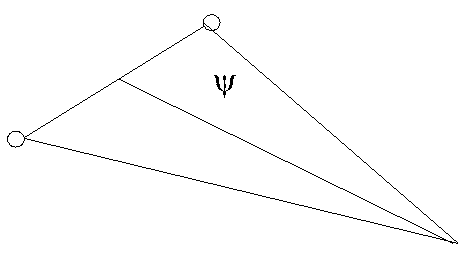
\includegraphics[width=.5\textwidth]{img/13-1.png}
\end{figure}
 
З геометричних міркувань знаходимо
\begin{equation}
	u(P) = \dfrac{-q}{4\pi r\epsilon_0 \sqrt{1-2\dfrac{\epsilon}{r}\cos\psi+\left(\dfrac{\epsilon}{r}\right)^2}} + \dfrac{q}{4\pi r\epsilon_0 \sqrt{1+2\dfrac{\epsilon}{r}\cos\psi+\left(\dfrac{\epsilon}{r}\right)^2}}.
\end{equation}

Застосовуючи формулу Тейлора і нехтуючи членами другого порядку малості отримаємо
\begin{equation}
	\begin{aligned}
		u(P) &= -\frac{q}{4\pi\epsilon_0 r} \left( 1 + \frac{\epsilon}{r}\cos\psi\right) + \frac{q}{4\pi\epsilon_0 r} \left( 1 - \frac{\epsilon}{r}\cos\psi\right) = \\
		&= -\frac{2\epsilon q\cos \psi}{4\pi\epsilon_0 r^2} = - \frac{p\cos\psi}{4\pi\epsilon_0 r^2}.
	\end{aligned}
\end{equation}

Припустимо, що ми маємо поверхню $S$ на якій розташовані диполі. Нехай $\mu(M): S \to \RR$ --- щільність моментів цих диполів. Тоді для кожної елементарної частини поверхні $\diff S$ момент диполів $\diff p$ дорівнює $\diff p = \mu \diff S$. \medskip

Враховуючи принцип суперпозиції потенціал електростатичного поля від такої зарядженої поверхні можна обчислити
\begin{equation}
	u(P) = -\Iint_S \frac{\cos\psi}{4\pi\epsilon_0 r^2} \diff p = - \Iint_S \mu(M) \frac{\cos\psi}{4\pi\epsilon_0 |MP|^2} \diff S_M.
\end{equation}
Де $|MP|$ ---відстань між точками $M$ і $P$. 

\begin{definition}[потенціалу подвійного шару]
	Оскільки на поверхні тіла орієнтація вісі диполя направлена по нормалі $n$ до поверхні, то потенціал електростатичного поля диполів поверхні буде мати вигляд інтегралу
	\begin{equation}
		u(P) = \frac{1}{4 \pi \epsilon_0} \Iint_S \mu(M) \frac{\partial}{\partial n} \frac{1}{|MP|} \diff S_M,
	\end{equation}
	який називається \it{потенціалом подвійного шару}.
\end{definition}

\subsubsection{Електричне поле в діелектриках}

Якщо діелектрик внести в електричне поле, то це поле і сам діелектрик змінює свої властивості. Ці зміни відбуваються за рахунок поляризації диполів, які заповнюють діелектрик, тобто під дією електричного поля орієнтуються в певному напрямку (до внесення поля їх розташування було хаотичне) і тим самим вносять зміни в зовнішнє електричне поле. 

\begin{definition}[електричної індукції]
	\it{Електрична індукція} поля в діелектрику визначається формулою 
	\begin{equation}
		\vecf D = \epsilon_0 \vecf E + \vecf P,
	\end{equation}
\end{definition}
де 	$\vecf P$ називають вектором \it{поляризації діелектриків} та для широкого класу діелектриків вектор $\vecf P$ можна записати у вигляді
\begin{equation}
	\vecf P = \epsilon_0 \chi \vecf E,
\end{equation}
	$\chi$ --- діелектрична сприйнятливість діелектрика. 


Таким чином електричну індукцію в діелектрику можна обчислити за формулою 
\begin{equation}
	\vecf E = \epsilon_a \vecf E,
\end{equation}
де
\begin{equation}
	\epsilon_a = \epsilon_0 (1 + \chi).
\end{equation}

Теорема Гауса для вектора електричної індукції записується у вигляді
\begin{equation}
	\Oiint_S D_n \diff S = \Iiint_\Omega \rho \diff \Omega.
\end{equation}

Враховуючи $\vecf E = \epsilon_a \vecf E$ та потенціальність вектора напруженості електричного поля будемо мати 
\begin{th_equation}[електростатики для діелектрика]
	\begin{equation}
		\nabla \cdot (\epsilon_a \nabla u) = - \rho.
	\end{equation}
\end{th_equation}

Розглянемо деякі наслідки теореми Гауса для граничних режимів:
\begin{itemize}
	\item Якщо двостороння поверхня $S$ діелектрика заряджена поверхневою щільністю $\sigma$, а в кожній точці поверхні заданий вектор нормалі $\vec n$, то з теореми Гауса випливає наслідок
	\begin{equation}
		\left. \left( \frac{\partial u}{\partial n} \right) \right|_{S^+} - \left. \left( \frac{\partial u}{\partial n} \right) \right|_{S^-} = - \left. E_n \right|_{S^+} + \left. E_n \right|_{S^-} = -\frac{\sigma}{\epsilon_0}.
	\end{equation}
	де знаком ``+'' позначені граничні значення нормальної похідної потенціалу зі сторони додатного значення нормалі, знаком ``-'' --- граничны значення потенцыалу з протилежного боку. \medskip

	Таким чином нормальна похідна потенціалу електростатичного поля, або нормальна складова напруженості електростатичного поля має розрив при переході через заряджену поверхню діелектрика.

	\item Якщо діелектрик з щільністю поверхневих зарядів примикає до провідника, то в провіднику електричне поле відсутнє, тобто потенціал дорівнює константі таким чином з попереднього наслідку потенціал на поверхні діелектрика задовольняє співвідношення 
	\begin{equation}
		\left. \left( \frac{\partial u}{\partial n} \right) \right|_{S^+} = - \left. E_n \right|_{S^+} = -\frac{\sigma}{\epsilon_+}.
	\end{equation}

	\item Якщо вздовж деякої поверхні $S$ межують два однорідних діелектрика з діелектричними сталими $\epsilon_+$, $\epsilon_-$ відповідно, то згідно моделі Фарадея, поверхня контакту є провідною у продовжному напрямку. З кожного боку на поверхні діелектриків має місце певна щільність зарядів $\sigma_+$, $\sigma_-$ відповідно, але сумарне значення цих щільностей дорівнює нулю, тобто
	\begin{equation}
		-\epsilon_+ E_{n^+} + \epsilon_- E_{n^-} = \epsilon_+ \left. \left( \frac{\partial u}{\partial n}\right)\right|_{S^+} - \epsilon_- \left. \left( \frac{\partial u}{\partial n}\right)\right|_{S^-} = 0.
	\end{equation}
\end{itemize}

\subsubsection{Постановка основних граничних задач електростатики}

Нехай у просторі задана деяка система провідників у вигляді заряджених поверхонь
\begin{equation}
	S = \Bigsqcup_{i = 1}^N S_i
\end{equation}
розміщених в деякому діелектрику. На кожному провіднику (поверхні) заданий потенціал $\left. U\right|_{S_i} = U_i = \const$. Необхідно визначити потенціал електростатичного поля в усіх точках простору. \medskip

У випадку, якщо у просторі відсутні додаткові заряди окрім заряджених поверхонь, то шуканий потенціал електростатичного поля задовольняє рівнянню Лапласа. Таким чином гранична задача приймає вигляд:
\begin{system}
    \label{eq:first-electrostatics-boundary-problem-homogeneous}
	& \Delta U = 0, \quad x \in \RR^3 \setminus S, \\
	& \left. U \right|_{S_i} = U_i, \quad i = \overline{1,N}, \\
	& \Lim_{|x| \to \infty} U = 0.
\end{system}

У випадку, якщо провідники розташовані у неоднорідному діелектрику у якому з щільністю $\rho$ розподілені вільні заряди, то гранична задача буде мати вигляд:
\begin{system}
    \label{eq:first-electrostatics-boundary-problem-heterogeneous}
	& \nabla \cdot (\epsilon_a(x) \nabla U) = - \rho(x), \quad  x \in \RR^3 \setminus S, \\
	& \left. U\right|_{S_i} = U_i, \quad i = \overline{1,N}, \\
	& \Lim_{|x| \to \infty} U = 0.
\end{system}

\begin{definition}[першої граничної задачі електростатики]
    Граничні задачі \eqref{eq:first-electrostatics-boundary-problem-homogeneous} і \eqref{eq:first-electrostatics-boundary-problem-heterogeneous} називають \textit{першими граничними задачами електростатики}.
\end{definition}

В електростатиці розглядається і другий тип граничної задачі, коли на поверхні провідника задаються умови другого роду:
\begin{equation}
	\left. \frac{\partial U}{\partial n} \right|_{S_i} = - \frac{\sigma_i}{\epsilon_0}.
\end{equation}

Фізично це означає, що на поверхні $S_i$ задається щільність поверхневих зарядів $\sigma_i$. \medskip	

Гранична умова другого роду не є природною для задач електростатики, оскільки поверхнева щільність важко вимірюється. \medskip

Більш природна постановка є такою:
\begin{example}
	Нехай у просторі заповненому діелектриком з діелектричною сталою $\epsilon_s$ задана деяка система провідників у вигляді заряджених поверхонь
	\begin{equation}
		S = \Bigsqcup_{i = 1}^N S_i.
	\end{equation}

	На кожному провіднику (поверхні) відомий повний заряд провідника $e_i$. Необхідно визначити потенціал електростатичного поля в усіх точках простору.
\end{example}

З основного рівняння електростатики запишимо:
\begin{equation}
    \label{eq:second-electrostatics-boundary-problem-equation}
	\nabla \cdot (\epsilon_a \nabla U) = 0, \quad x \in \RR^3 \setminus S,
\end{equation}
на кожгому провіднику задамо $\left. U \right|_{S_i} = U_i = \const$, де $U_i$ --- невідомі величини. Умову повного заряду провідника запишемо у вигляді: 
\begin{equation}
    \label{eq:second-electrostatics-boundary-problem-boundary-conditions}
	\Oiint_{S_i} \epsilon_a \frac{\partial U}{\partial n} \diff S = -e_i,
\end{equation}
де інтегрування ведеться по довільній замкненій поверхні ${S_i}$, яка охоплює провідник.
Завершує постановку  умови затухання потенціалу на нескінченості
\begin{equation}
    \label{eq:second-electrostatics-boundary-problem-conditions-at-the-infinity}
	\Lim_{|x| \to \infty} U = 0.
\end{equation}

\begin{definition}[другої граничної задачі електростатики]
	Гранична задача \eqref{eq:second-electrostatics-boundary-problem-equation}--\eqref{eq:second-electrostatics-boundary-problem-conditions-at-the-infinity} називається \textit{другою граничною задачею електростатики}.
\end{definition}

\subsection{Математичні моделі магнітостатики}

Відомо що взаємодіють між собою не тільки електричні заряди але і електричні струми. Так наприклад два паралельних провідники, по яким протікають постійні електричні струми притягуються між собою, якщо струми мають однаковий напрям і відштовхуються, якщо струми мають протилежний напрям. Зокрема Ампером було встановлено, що сила взаємодії провідників розрахована на одиницю довжини провідника пропорційна величинам струмів в них $I_1$ та $I_2$ і обернено пропорційна відстані між паралельними провідниками $r$ та дорівнює
\begin{equation}
	f = \frac{\mu_0}{4 \pi} \frac{I_1 I_2}{r},
\end{equation}
де $\mu_0$ --- коефіцієнт магнітної проникливості. \medskip

Взаємодія струмів відбувається через поле яке називається магнітним, така назва поля виникла у зв'язку з тим, що як винайшов у 1820 році Ерстед, поле провідника постійного струму впливає на орієнтацію магнітної стрілки. \medskip

Таким чином можна зробити висновок, що заряди, які рухаються змінюють властивості оточуючого їх простору --- створюючи в ньому магнітне поле. Це поле проявляється в тому, що воно впливає на заряди, що рухаються в цьому полі (струми). \medskip

Подібно тому, як пробний точковий заряд використовувався нами для дослідження електричного поля, так для дослідження магнітного поля можна використовувати пробний струм, який циркулює в площинному замкненому контурі дуже малих розмірів. \medskip

Орієнтацію контуру в просторі будемо характеризувати за допомогою вектору нормалі до площини контуру, який обирається за правилом правого гвинта. (Якщо обходити контур, так, що область знаходиться ліворуч спостерігача, то нормаль орієнтована від ніг до голови спостерігача). Таку орієнтацію нормалі називають додатною. \medskip

Вносячи пробний контур у магнітне поле, ми спостерігаємо, що поле здійснює на контур орієнтуючу дію, встановлюючи її додатню нормаль у певному напрямі. Приймемо цей напрям за напрям поля у цій точці. Якщо повернути контур так, що напрям додатньої нормалі і напрям поля не співпадали, то виникає обертальний момент, який прагне повернути контур в рівноважне положення. Величина моменту у точці залежить від кута $\alpha$ між нормаллю і напрямом поля. І досягає найбільшого значення $M_{\text{max}}$ при $\alpha = \pi / 2$, при $\alpha = 0$ момент дорівнює нулю. Обертальний момент залежить як від властивостей поля в заданій точці так і від властивостей контуру. Так вносячи різноманітні пробні контури можна побачити, що $M_{\text{max}}$ пропорційний силі струму, що циркулює в контурі, і площі, яку охоплює контур і зовсім не залежить від форми контуру. 

\begin{definition}[магнітного моменту контуру]
	Таким чином дія магнітного поля на площинний контур визначається величиною $P_M = I S$, яку називають абсолютним значенням \it{магнітного моменту контуру}.
\end{definition}

Окрім сили току $I$ та площі $S$ пробний контур характеризується орієнтацією у просторі, тому магнітний момент слід розглядати, як вектор, напрям якого співпадає з напрямом одиничної нормалі, тому
\begin{equation}
	\vec p_M = I S \vec n.
\end{equation}

На пробні контури з різним значенням $p_M$ в даній точці поля діють різні обертальні моменти $M_{\text{max}}$. В той же час відношення $M_{\text{max}} / p$ для усіх контурів буде одне і теж саме і може бути прийняте за кількісну характеристику магнітного поля. 

\begin{definition}[індукції]
	Фізичну величину $B$, яка пропорційна цьому відношенню називають магнітною індукцією:
	\begin{equation}
		B \simeq \frac{M_{\text{max}}}{p_M}.
	\end{equation}
\end{definition}

Магнітна індукція --- векторна величина, напрям якої визначається рівноважним положенням нормалі пробного контуру, а рівняння вище визначає модуль вектору $\vecf B$.

\begin{definition}[напруженості магнітного поля]
	Поряд з вектором магнітної індукції $\vecf B$ розглядається також векторна величина $\vecf H$, яку називають \it{напруженістю магнітного поля}. Для вакууму та інших ізотропних середовищ, які не мають магнітних властивостей зв'язок між вектором магнітної індукції та вектором напруженості магнітного поля має вигляд. 
	
	\begin{equation}
		\vecf B = \mu \vecf H,
	\end{equation}
	тобто ці вектори колінеарні.
	Де 	$\mu = \const$ --- \it{магнітна проникливість середовища}, через $\mu_0$ будемо позначати магнітну проникливість вакууму.
\end{definition}

\subsubsection{Закон Біо-Савара}

Біо та Савар у 1820 році провели дослідження магнітних полів струмів різної форми та з'ясували, що напруженість магнітного поля в усіх випадках пропорційна силі струму, який створює магнітне поле, і доволі складним чином залежить від відстані до цієї точки. Експериментальні дані Біо Савара проаналізував Лаплас і встановив, що для елементу струму, який направлений вздовж вектора нескінченно малого зміщення $\diff \vec l$ і має величину $I$ величина напруженості магнітного поля $\diff \vecf H$ визначається за формулою:
\begin{equation}
	\diff \vecf H = \frac{1}{4 \pi} \frac{I \left(\diff \vec l \times \vec r\right)}{|r|^3},
\end{equation}
де $\vec r$ --- вектор, направлений від елементу струму до точки у якій обчислюється напруженість магнітного поля, $\vec a \times \vec b$ --- векторний добуток двох векторів.  \medskip

Виходячи з цієї формули легко обчислити поле прямого струму
\begin{equation}
	\begin{aligned}
		\left| \vecf H \right| &= \left| \Int_{-\infty}^\infty \diff \vecf H \right| = \frac{1}{4\pi} \Int_{-\infty}^\infty \frac{I \cdot |\diff l| \cdot |r| \cdot \sin \alpha}{|r|^3} = \\
		&= \frac{1}{4\pi} \Int_0^\pi \frac{I \cdot |r| \cdot \sin \alpha}{|r|^2 \cdot \sin \alpha} \diff \alpha = \frac{I}{4\pi} \Int_0^\pi \frac{\diff \alpha}{|r|} = \\
		&= \frac{I}{4\pi b} \Int_0^\pi \sin \alpha \diff \alpha = \frac{I}{2\pi b},
	\end{aligned}
\end{equation}
де всі величини зображені на наступному рисунку:
\begin{figure}[H]
	\centering
%	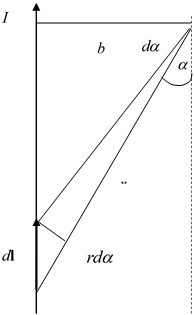
\includegraphics[]{img/13-2.png}
\end{figure}

При цьому вектор $\vec H$ має напрям по дотичній до концентричних кіл з центром у точці проходження струму і орієнтований за правилом правого гвинта.

\subsubsection{Циркуляція вектора напруженості магнітного поля}

Нехай ми маємо магнітне поле з вектором магнітної напруженості $\vecf H$, який є функцією точки простору. 

\begin{definition}[циркуляції векторного поля]
	\it{Циркуляцією} векторного поля $\vecf H$ будемо називати величину
	\begin{equation}
		\Oint_C \langle \vecf H, \diff \vec l \rangle
	\end{equation}
	де $C$ --- замкнений контур в просторі. 
\end{definition}

Обчислимо циркуляцію вектора магнітної напруженості вздовж будь-якого замкненого плоского контуру, що охоплює деякий прямий струм, ортогональний до площини контуру:
\begin{figure}[H]
	\centering
%	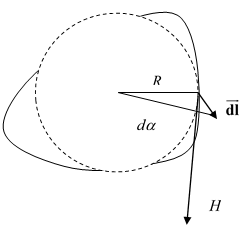
\includegraphics[width=.5\textwidth]{img/13-3.png}
\end{figure}

Враховуючи, формулу $\left| \vecf H \right| = I / 2 \pi b$, можна записати, що
\begin{equation}
	\langle \vecf H, \diff \vec l \rangle = \frac{I}{2 \pi R} R \diff \alpha.
\end{equation}

Таким чином циркуляція
\begin{equation}
	\Oint_C \langle \vecf H, \diff \vec l \rangle = \frac{I}{2 \pi} \Oint_C \diff \alpha = I.
\end{equation}

У випадку, коли контур охоплює декілька струмів, то ця формула узагальнюється:
\begin{equation}
	\Oint_C \langle \vecf H, \diff \vec l \rangle = \Sum I.
\end{equation}

У випадку, коли струми розподілені у просторі з деякою щільністю $\vec j$, то величина струму, що протікає через довільну поверхню $S$ може бути записаний у вигляді
\begin{equation}
	I = \Int_S \vec j_n \diff S.
\end{equation}

Таким чином маємо 
\begin{law}[циркуляції магнітного поля]
	\begin{equation}
		\Oint_C \langle \vecf H, \diff \vec l \rangle = \Iint_S \vec j_n \diff S
	\end{equation}
\end{law}

У цій формулі $C$ --- довільний контур у просторі, $S$ --- довільна поверхня, яка спирається на контур $C$. \medskip

Використовуючи формулу Стокса, отримаємо 
\begin{equation}
	\Iint_S \left(\nabla \times \vecf H\right)_n = \Iint_S \vec j_n \diff S.
\end{equation}

Враховуючи, що поверхня $S$ обрана довільним чином можемо записати 
\begin{th_equation}[магнітостатики]
	Воно є частинним випадком третього рівняння поля:
	\begin{equation}
        \label{eq:magnetostatics-equation-third-field-equation}
		\nabla \times \vecf H = \vec j.
	\end{equation}
\end{th_equation}
Порівнюючи закон циркуляції магнітного поля у вакуумі та формулу
\begin{equation}
	\Oint_C \langle \vecf E, \diff \vec l \rangle = 0
\end{equation}
для електричного поля, бачимо між цими полями суттєву різницю. Так циркуляція по замкненому контуру електричного поля дорівнює нулю, а значить це поле потенціальне, магнітне поле не є потенціальним, його називають вихровим. \medskip

Другою особливість магнітного поля полягає в тому, що лінії магнітної індукції, а значить і лінії напруженості магнітного поля у вакуумі завжди замкнені, що свідчить про відсутність у природі магнітних зарядів. Замкненість ліній магнітної індукції та ліній напруженості магнітного поля означають, що потік векторного поля магнітної індукції через будь-яку замкнену поверхню дорівнює нулю. Тобто
\begin{equation}
	\Oiint_S \vecf B_n \diff S = 0.
\end{equation}

З формули Остроградського Гауса отримаємо ще одне рівняння магнітостатики, яке є частинним випадком другого рівняння теорії поля:
\begin{equation}
	\nabla \cdot \vecf B = 0,
\end{equation}
або, враховуючи $\vecf B = \mu \vecf H$,
\begin{equation}
    \label{eq:magnetostatics-equation-second-field-equation}
	\nabla \cdot \left(\mu_0 \vecf H\right) = 0.
\end{equation}

Таким чином рівняння магнітостатики для вакууму представляють собою систему з другого і третього рівнянь поля.

\subsubsection{Магнітне поле в середовищі}

Деякі речовини мають здатність до намагнічування: тобто під дією прикладеного до них магнітного поля можуть отримувати магнітний момент. Одні речовини намагнічуються сильніше, інші слабкіше, таки речовини називаються магнетиками. \medskip

Для магнетиків розміщених у зовнішньому магнітному полі утворюється додаткове магнітне поле і сумарне магнітне поле визначається як
\begin{equation}
	\vecf B = \vecf B_i + \vecf B',
\end{equation}

де $\vecf B_i$ --- зовнішнє магнітне поле обумовлене електричним струмом чи іншим чинником, $\vecf B'$ --- додаткове магнітне поле середовища здатного до намагнічування.  \medskip

Для пояснення явища намагнічування середовищ Ампер припустив, що в молекулах тіла циркулюють кругові струми. Кожний струм має магнітний момент і створює в оточуючому просторі магнітне поле. Якщо зовнішнє магнітне поле відсутнє, то молекули розташовані хаотично і результуюче поле дорівнює нулю.  В результаті хаотичної орієнтації магнітних моментів, сумарний магнітний момент  тіла також рівний нулю. Під дією зовнішнього поля моменти молекул сприймають переважну орієнтацію в одному напрямку, за рахунок чого магнетик намагнічується і його сумарний магнітний момент становиться відмінним від нуля. Магнітні поля окремих молекулярних струмів вже не компенсують одне одного, а утворюють додаткове магнітне поле $\vecf B'$:
\begin{figure}[H]
	\centering
	%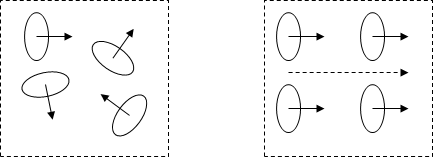
\includegraphics[]{img/13-4.png}
\end{figure}

\begin{definition}[вектору намагнічування]
	Намагнічування магнетика природно характеризувати магнітним моментом одиниці об'єму. Цю величину називають \it{вектором намагнічування} і позначають $\vecf J$.
\end{definition}

Дослідним шляхом встановлено, що вектор намагнічування $\vecf J$ зв'язаний з напруженістю зовнішнього поля у точці співвідношенням
\begin{equation}
	\vecf J = \chi \vecf H.
\end{equation}

\begin{definition}[магнітної сприйнятливості речовини]
    Тут $\chi$ --- безрозмірна величина, яку називають \it{магнітною сприйнятливістю речовини}.
\end{definition}

В залежності від знаку і величини магнітної сприйнятливості $\chi$ усі магнетики поділяються на класи:
\begin{itemize}
	\item Діамагнетики --- для яких $\chi$ --- мала за абсолютною величиною і від'ємна.
	\item Парамагнетики --- для яких $\chi$ --- мала за величиною і додатна.
	\item Феромагнетики --- для яких $\chi$ --- додатна і досягає дуже великих значень.
\end{itemize}

Таким чином враховуючи $\vecf B = \vecf B_i + \vecf B'$ та $\vecf J = \chi \vecf H$, можемо записати, що зв'язок між вектором магнітної індукції та вектором напруженості магнітного поля для магнетиків матиме вигляд $\vecf H = \vecf B / \mu_0 - \vecf J$, або $\vecf H = \vecf B / \mu_0 - \chi \vecf H$, звідки маємо 
\begin{equation}
	\vecf H = \frac{\vecf B}{\mu_0 (1 + \chi)} = \frac{\vecf B}{\mu_\alpha},
\end{equation}
де $\mu_\alpha = \mu_0 (1 + \chi)$. \medskip

Таким чином для магнетиків рівняння магнітостатики приймають вигляд другого і третього рівняння поля \eqref{eq:magnetostatics-equation-second-field-equation}, \eqref{eq:magnetostatics-equation-third-field-equation}, де вектор магнітної індукції і напруженість магнітного поля зв'язані між собою останнім співвідношенням.

\subsubsection{Граничні умови для магнітного поля}

При переході через границю розділу двох магнетиків з різними магнітними проникливостями $\mu_1$ і $\mu_2$ силові лінії магнітного поля відчувають переломлення. Для з'ясування, яким чином  відбувається переломлення ліній поля необхідно встановити яким чином переломлюються нормальні та тангенціальні складові на границі. Отримання граничних умов здійснюються за допомогою теореми Гауса для магнітного поля і теореми про циркуляції магнітного поля. \medskip

Для нормальних складових вектора магнітної індукції $\vecf B$, теорема Гауса дає
\begin{equation}
	\langle \vecf B_2, \vec n_2 \rangle S_2 + \langle \vecf B_1, \vec n_1 \rangle S_1 = 0,
\end{equation}
де $S_1 = S_2$:
\begin{figure}[H]
	\centering
%	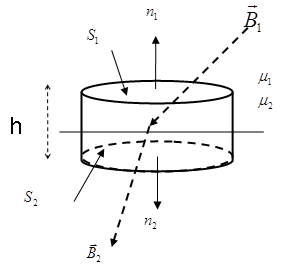
\includegraphics[width=.5\textwidth]{img/13-5.png}
\end{figure}

Потік магнітної індукції $\vecf B$ через бокову поверхню циліндру при $h \to 0$ стає нескінченно малим і їм можна нехтувати. Таким чином
\begin{equation}
	\left. \langle \vecf B_1, \vec n_1 \rangle \right|_S = \left. \langle \vecf B_2, \vec n_1 \rangle \right|_S.
\end{equation}

Тобто на границі розділу двох магнетиків виконується умова неперервності нормальної складової вектора магнітної індукції $\vecf B_n$. \medskip

Припустимо, що на границі, що розділяє два магнетики не тече поверхневий електричний струм, тоді згідно до теореми про циркуляцію напруженості магнітного поля, будемо мати
\begin{equation}
	\langle \vecf H_1, \tau \rangle a_1 - \langle \vecf H_2, \tau \rangle a_2 = 0,
\end{equation}
де $a_1 = a_2$ --- горизонтальні елементи контуру інтегрування:
\begin{figure}[H]
	\centering
%	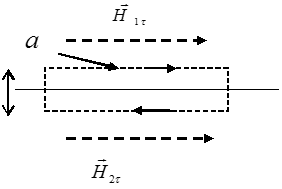
\includegraphics[width=.5\textwidth]{img/13-6.png}
\end{figure}

Інтеграл по вертикальним складовим контуру при $h \to 0$ прямує до нуля. \medskip

Таким чином дотичні (тангенціальні) складові напруженості магнітного поля неперервні при переході через границю двох магнетиків, а відповідна гранична умова приймає вигляд:
\begin{equation}
	\left. \vecf H_{1\tau} \right|_S = \left. \vecf H_{2\tau} \right|_S
\end{equation}

Якщо врахувати зв'язок між векторами магнітної індукції і вектором напруженості магнітного поля, то можна записати
\begin{align}
	\mu_2 \left. \vecf B_{1\tau} \right|_S &= \mu_1 \left. \vecf B_{2\tau} \right|_S, \\
	\mu_1 \left. \vecf H_{1n} \right|_S &= \mu_2 \left. \vecf H_{2n} \right|_S.
\end{align}

Якщо на поверхні, що розділяє два магнетики протікає електричний струм з лінійною щільністю $\vec i$, то тоді замкнений контур охоплює поверхневий струм і поверхневий інтеграл обчислюється з використанням третього рівняння поля. В результаті будемо мати умову:
\begin{equation}
	\left. \vecf H_{1\tau} \right|_S - \left. \vecf H_{2\tau} \right|_S = \langle \vec i, \vec N \rangle
\end{equation}
де $\vec N = \tau \times \vec n$ --- векторний добуток дотичного вектора $\tau$ та вектора нормалі $\vec n$, до поверхні $S$, що розділяє два магнетики.

\subsubsection{Векторний потенціал}

Нагадаємо систему рівнянь магнітостатики для магнетиків.
\begin{system}
	& \nabla \cdot \vecf B = 0, \\
	& \nabla \times \vecf H = \vec j, \\
	& \vecf B = \mu_a \vecf H.
\end{system}

З другого рівняння випливає, що $\nabla \cdot \vec j = 0$, оскільки $\nabla \cdot (\nabla \times \vecf H) = 0$. \medskip

Умова соленоїдальності векторного поля $\vecf B$ (перше рівняння) виконано коли
\begin{equation}
	\vecf B = \nabla \times \vecf A,
\end{equation}
де $\vecf A$ --- векторний потенціал, що залежить від координат точок простору. Оскільки $\nabla \times (\nabla \psi) = 0$, то векторне поле магнітної індукції не зміниться, якщо замість вектора $A$ узяти $A_1 = A + \nabla \psi$, де $\psi$ --- довільна скалярна функція. Таким чином векторний потенціал для поля магнітної індукції $\vecf B$ не визначається однозначно. У зв'язку з чим векторний потенціал $\vecf A$ можна підпорядкувати додатковій умові
\begin{equation}
	\nabla \cdot \vecf A = 0.	
\end{equation}

\begin{remark}
	Виконання цієї умови завжди можна забезпечити вибором функції $\psi$.
\end{remark}

Використаємо представлення $\vecf B = \nabla \times \vecf A$, тоді з другого та третього рівняння отримаємо
\begin{equation}
	\nabla \times \nabla \times \vecf A = \vec j \mu_a.	
\end{equation}

Врахуємо, що
\begin{equation}
	\nabla \times \nabla \times \vecf A = \nabla (\nabla \cdot \vecf A)	- \Delta \vecf A = \mu_a \vec j.
\end{equation}

Використовуючи умову $\nabla \cdot \vecf A = 0$, отримаємо рівняння для векторного потенціалу
\begin{equation}
	\Delta \vecf A = - \mu_a \vec j.	
\end{equation}

Таким чином система рівнянь магнітостатики зводиться до векторного рівняння Пуассона для векторного потенціалу.

\end{document}